\newpage
\subsubsection{Les écrans}
\paragraph{Vue générale}

Utilisateur peut interagir avec Tableau de Bord via l'application {\nomApplication}. L'application {\nomApplication} peut transmettre des informations à Utilisateur par l'intermédiaire de l'écran du Smartphone. \newline

La figure \ref{schemaMAE} représente les navigations possibles entre les différents écrans proposés par l'IHM. Ces enchaînements sont représentés par un diagramme d'états-transitions UML. \\
Chaque écran est représenté par un état (rectangle arrondi sur la figure). Les transitions indiquées par les flèches représentent une navigation d'un écran à l'autre en précisant l'événement logique du contexte (cf. chapitre \ref{interfaces_logiques}) qui active la transition. Cela correspond généralement à des interactions de Utilisateur sur l'IHM qui génère l'événement correspondant.
\newline

Certaines transitions ne sont pas franchies sur des événements logiques, ce sont :
\begin{itemize}
    \item Les événements de temporisation (le mot-clef « after » est alors noté sur la transition) : la transition doit être sensibilisée pendant une certaine durée pour être franchie.
    \item Des conditions qui deviennent vraies (la condition est alors exprimée entre crochets).
\end{itemize}

\begin{figure}[ht] 
    \centering
    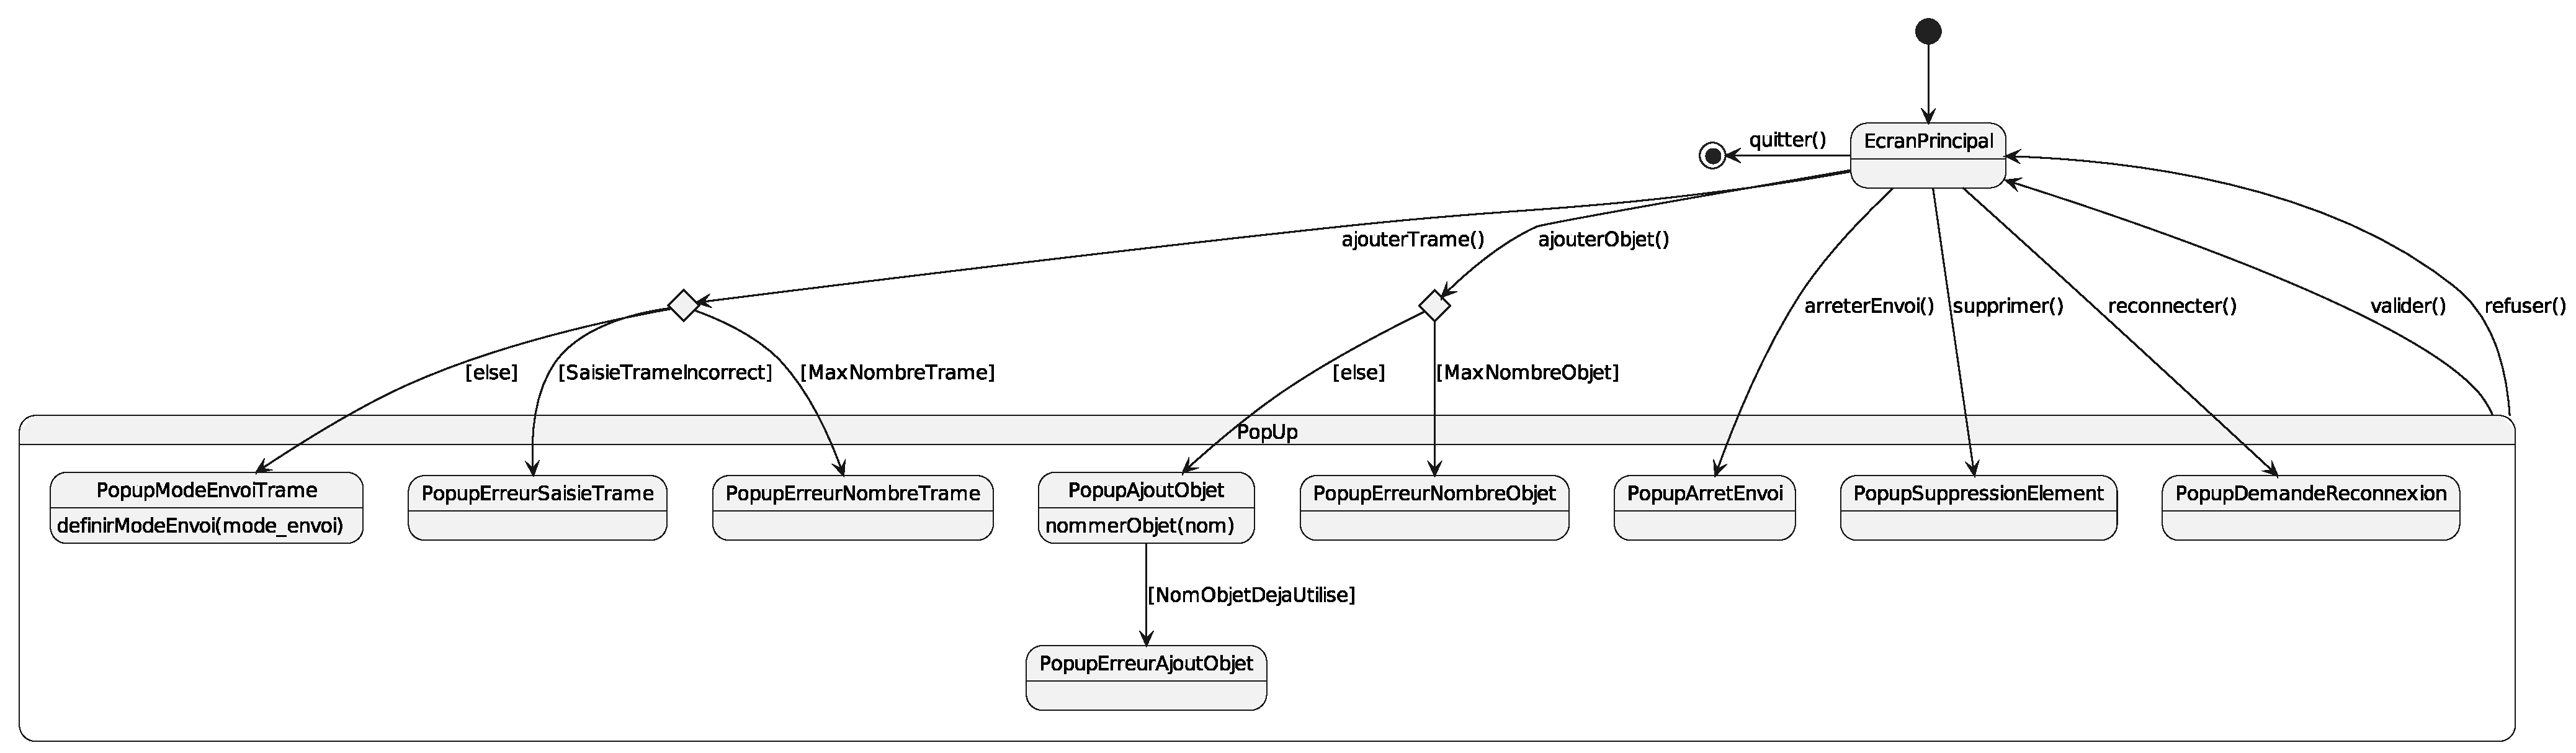
\includegraphics[width=16cm]{../schemas/MAE}
    \captionsetup{justification=centering}
    \caption{Enchaînement entre les écrans de l'IHM représenté par un diagramme états-transitions UML}
    \label{schemaMAE}
\end{figure}

\newpage

L'état initial de création de l'IHM est représenté par le disque de couleur noire. 
Après le lancement du système, l'IHM démarre avec l'écran {\guillemetleft} EcranPrincipal {\guillemetright}. 
Le disque de couleur noire entouré par un cercle correspond à la fin d'un enchaînement. 
Lorsqu'un enchaînement est fini, l'IHM s'éteint.
\newline
\newline
\`A partir de EcranPrincipal, Utilisateur peut réaliser différentes actions, qui déclencheront l'apparition de pop-up (afficherPopUp(id\_popup)). Utilisateur peut à tout moment revenir à EcranPrincipal (refuser()).
\newline
\newline
Dans le cas d'un ajout d'objet (ajouterObjet()), l'IHM affiche PopupAjoutObjet (afficherPopUp(id\_popup)). Utilisateur nomme l'objet (nommerObjet(nom)), il doit appuyer sur le bouton {\guillemetleft} Ajouter {\guillemetright} nommé [validerAjoutObjet] dans la figure \ref{ecran_ajout_objet}. Cela correspond à la fonction {\guillemetleft} valider() {\guillemetright} de la figure \ref{schemaMAE}. Si Utilisateur ne souhaite pas choisir de nom, l'application {\nomApplication} en fournit un par défaut (voir section \ref{dictionnaire}).
\newline
\newline
Dans le cas où Utilisateur saisit un nom d'objet qui est déjà utilisé par un autre objet, l'IHM affiche le pop-up d'erreur PopUpErreurAjoutObjet (afficherPopUp(id\_popup)). Ce pop-up contient une phrase qui informe Utilisateur de la source de l'erreur. Tant que Utilisateur n'aura pas modifié le nom de l'objet, il ne pourra pas l'ajouter à la liste de l'application CANdroid.
\newline
\newline
Dans le cas d'un ajout de trame (ajouterTrame()), l'IHM affiche PopupModeEnvoiTrame (afficherPopUp(id\_popup)) pour définir le mode d'envoi (definirModeEnvoi(mode\_envoi)) de la trame à ajouter. Utilisateur doit appuyer sur le bouton {\guillemetleft} Ajouter {\guillemetright} nommé [validerModeEnvoi] dans la figure \ref{ecran_mode_trame_envoi}. Cela correspond à la fonction {\guillemetleft} valider() {\guillemetright} de la figure \ref{schemaMAE} qui permet à Utilisateur de confirmer son choix.
\newline
\newline
Dans le cas où Utilisateur saisit une trame qui ne correspond pas au format utilisé par l'application CANdroid, l'IHM affiche le pop-up d'erreur PopupErreurSaisieTrame (afficherPopUp(id\_popup)). Pour fermer ce pop-up, Utilisateur doit appuyer sur le bouton [fermerErreurTrame]. Il pourra par la suite modifier le format de la trame saisie afin de pouvoir l'ajouter correctement.
\newline
\newline
Dans le cas où le nombre maximum de trames ou d'objets est atteint, l'IHM affiche respectivement les pop-ups d'erreur PopupErreurNombreTrame (afficherPopUp(id\_popup)) et PopupErreurNombreObjet (afficherPopUp(id\_popup)). Ces pop-ups contiennent un message d'erreur qui informe Utilisateur de la nature de l'erreur. Utilisateur peut simplement fermer le pop-up en cliquant sur la croix située en haut à droite. Cette action le ramènera sur EcranPrincipal. Dans la figure \ref{ecran_erreur_ajout_nombre_trame}, la croix est identifiée par [fermerErreurNombreTrame], tandis que dans la figure \ref{ecran_erreur_ajout_nombre_objet} elle est identifiée par [fermerErreurNombreObjet].
\newpage
Dans le cas d'une suppression d'élément (supprimer()), l'IHM affiche PopupSuppressionElement (afficherPopUp(id\_popup)). Le pop-up affiche la liste des éléments sélectionnés, Utilisateur doit appuyer sur le bouton {\guillemetleft} Supprimer {\guillemetright} nommé [validerSuppressionElement] dans la figure \ref{ecran_suppression_element}. Cela correspond à la fonction {\guillemetleft} valider() {\guillemetright} de la figure \ref{schemaMAE} qui permet à Utilisateur de confirmer son choix.
\newline
\newline
Dans le cas d'un arrêt de l'envoi de trames (arreterEnvoiTrames()), l'IHM affiche PopupArretEnvoi (afficherPopUp(id\_popup)). Utilisateur doit appuyer sur le bouton {\guillemetleft} Oui {\guillemetright} nommé [validerArretEnvoi] dans la figure \ref{ecran_arret_envoi_trame}, ou sur le bouton {\guillemetleft} Non {\guillemetright} nommé [annulerArretEnvoi] dans la même figure. Cela correspond respectivement aux fonctions {\guillemetleft} valider() {\guillemetright} et {\guillemetleft} refuser() {\guillemetright} de la figure \ref{schemaMAE} qui permet à Utilisateur de confirmer ou annuler son choix.
\newline
\newline
Dans le cas d'une perte de connexion, si Utilisateur souhaite se reconnecter (reconnecter()), l'IHM affiche PopupDemandeReconnexion(afficherPopUp(id\_popup)). Utilisateur choisit de se reconnecter en appuyant sur le bouton {\guillemetleft} Oui {\guillemetright} nommé [validerReconnexion] dans la figure \ref{ecran_demande_reconnexion}, ou sur le bouton {\guillemetleft} Non {\guillemetright} nommé [annulerReconnexion] dans la même figure. Cela correspond respectivement aux fonctions {\guillemetleft} valider() {\guillemetright} et {\guillemetleft} refuser() {\guillemetright} de la figure \ref{schemaMAE} qui permet à Utilisateur de confirmer ou annuler son choix.

\newpage
\paragraph{EcranPrincipal}

\vspace{1cm}
\begin{minipage}{1\linewidth}
    \centering
    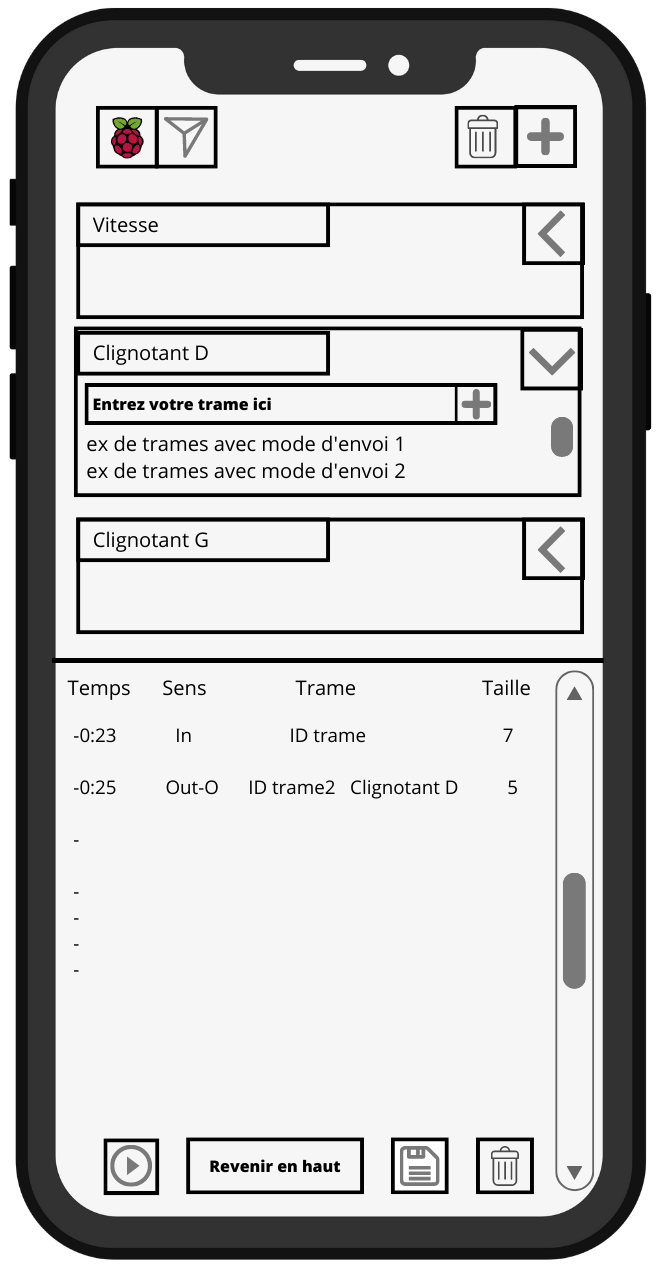
\includegraphics[width=0.45\textwidth]{sections/3_Exigences_specifiques/1_IHM/ihm/ecranPrincipal.png}
    \captionsetup{justification=centering}
    \captionof{figure}{Affichage général de EcranPrincipal}
    \label{ecran_principal}
\end{minipage}\hfill
\newline
\newline
EcranPrincipal se décompose en deux parties. La partie haute permet de déclencher des interactions avec Tableau de Bord tandis que la partie basse correspond au sniffer CAN.
\medskip

\newpage
\paragraph{Partie haute de l'écran}
\medskip
La partie {\guillemetleft} envoi {\guillemetright} (partie haute de l'écran) permet d'intéragir avec Tableau de Bord. On y observe l'état de la connexion au programme {\nomLogiciel}. On peut ajouter ou supprimer des objets, et dans ces mêmes objets, ajouter ou supprimer des trames. Enfin, on peut y ordonner l'envoi de trames. 
\newline
\newline
\textbf{Connexion : } \\

Lors du démarrage de l'application {\nomApplication}, la connexion avec le programme {\nomLogiciel} s'initialise automatiquement et continue en tâche de fond de l'application. Une connexion valide est représentée par l'icône de framboise (bouton [connexion]) en haut à gauche. Si la connexion ne s'est pas correctement déroulée, l'icône est grisée et barrée. Ainsi, au lancement de l'application {\nomApplication}, l'icône est d'abord grisée et barrée (voir figure \ref{ecran_principal_non_connecte}), puis, elle se colore si la connexion aboutit en moins de 3 secondes (voir figure \ref{ecran_sans_objet}). Si la connexion n'aboutit pas, Utilisateur peut demander à recommencer en cliquant sur le bouton [connexion] (dont l'icône est grisée et barrée). Un pop-up s'affiche et demande si l'on souhaite une reconnexion ou non au programme {\nomLogiciel} (voir figure \ref{ecran_principal_demande_reconnexion}). L'application {\nomApplication} peut être utilisée sans connexion. Dans ce cas, l'icône de framboise reste grisée et barrée. Le bouton [lancerEnvoi] est de couleur noire sur fond gris foncé pour indiquer qu'il est impossible d'envoyer des trames sur le bus CAN. De même pour le sniffer où le bouton [play] n'est pas cliquable. S'il est vide alors un message nous informe qu'il n'y a pas de trames sur le bus (voir figure \ref{ecran_principal_non_connecte}). 

\begin{minipage}{0.5\linewidth}
    \centering
    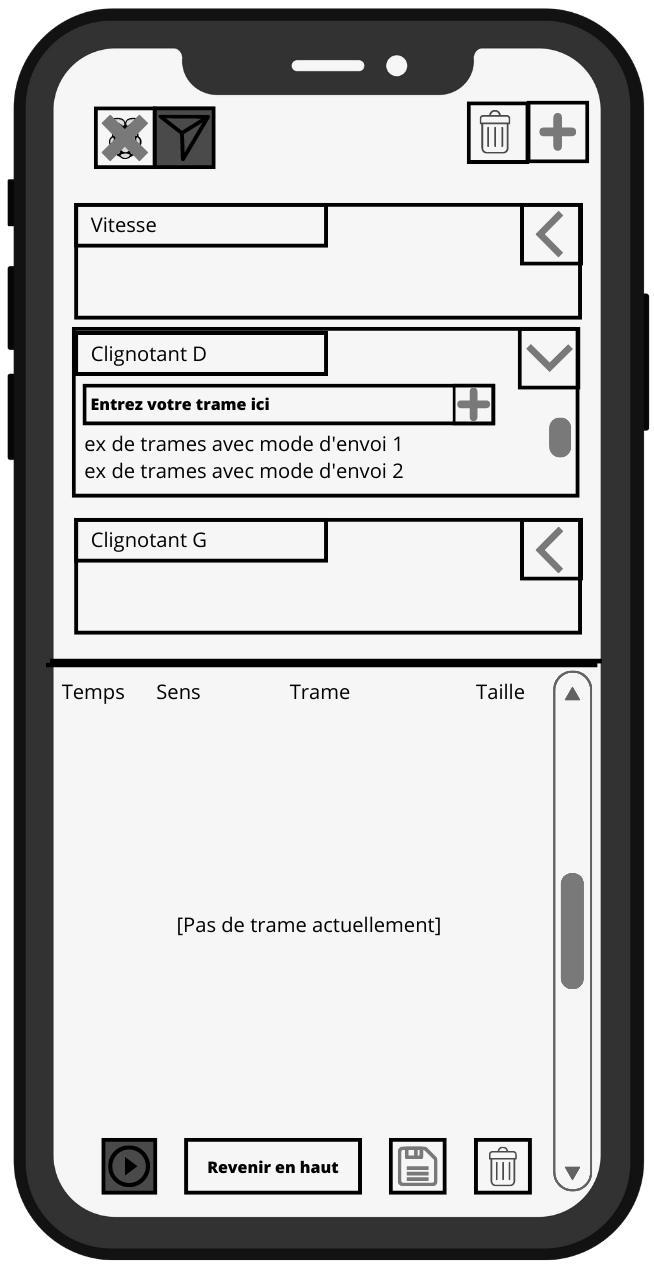
\includegraphics[width=0.7\textwidth]{sections/3_Exigences_specifiques/1_IHM/ihm/ecranPrincipalNonCo.png}
    \captionsetup{justification=centering}
    \captionof{figure}{Affichage de EcranPrincipal \newline non connecté}
    \label{ecran_principal_non_connecte}
\end{minipage}\hfill
\begin{minipage}{0.5\linewidth}
    \centering
    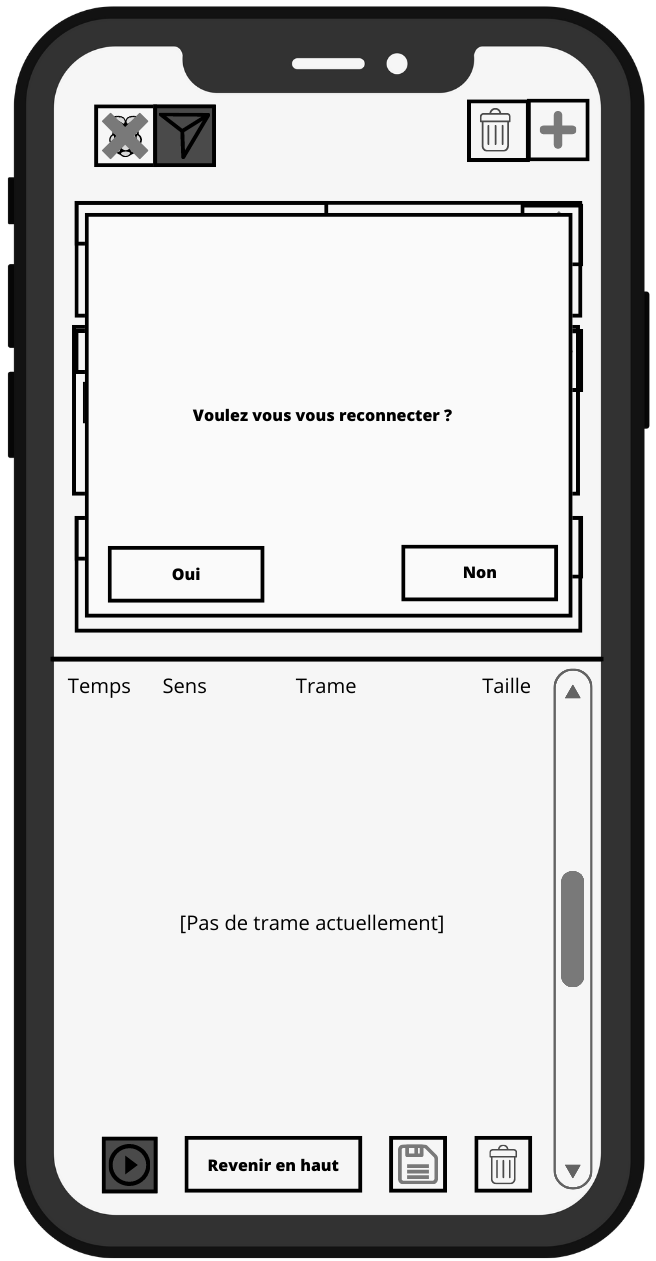
\includegraphics[width=0.7\textwidth]{sections/3_Exigences_specifiques/1_IHM/ihm/ecranReconnexion.png}
    \captionsetup{justification=centering}
    \captionof{figure}{Affichage de PopupDemandeReconnexion}\label{ecran_principal_demande_reconnexion}
\end{minipage}

\newpage
\textbf{Objet : } \\
\newline
Les objets sont matérialisés sur l'application {\nomApplication} par un rectangle (voir figure \ref{ecran_principal}). Ce rectangle comprend un sous-rectangle avec le nom de l'objet en haut à gauche et, à droite, une flèche déroule le menu de l'objet (bouton [deplierMenuObjet] ou [replierMenuObjet] pour l'effet inverse) pour afficher les trames déjà ajoutées dans cet objet. \newline \\
Les objets sont conservés d'une utilisation à l'autre sur l'application {\nomApplication}. Ils sont triés du plus récent en haut au plus ancien.
Lorsqu'il n'y a pas d'objet, un texte l'indique par un message d'information (voir figure \ref{ecran_sans_objet}). 
\vspace{0.5cm}

\begin{minipage}{0.9\linewidth}
    \centering
    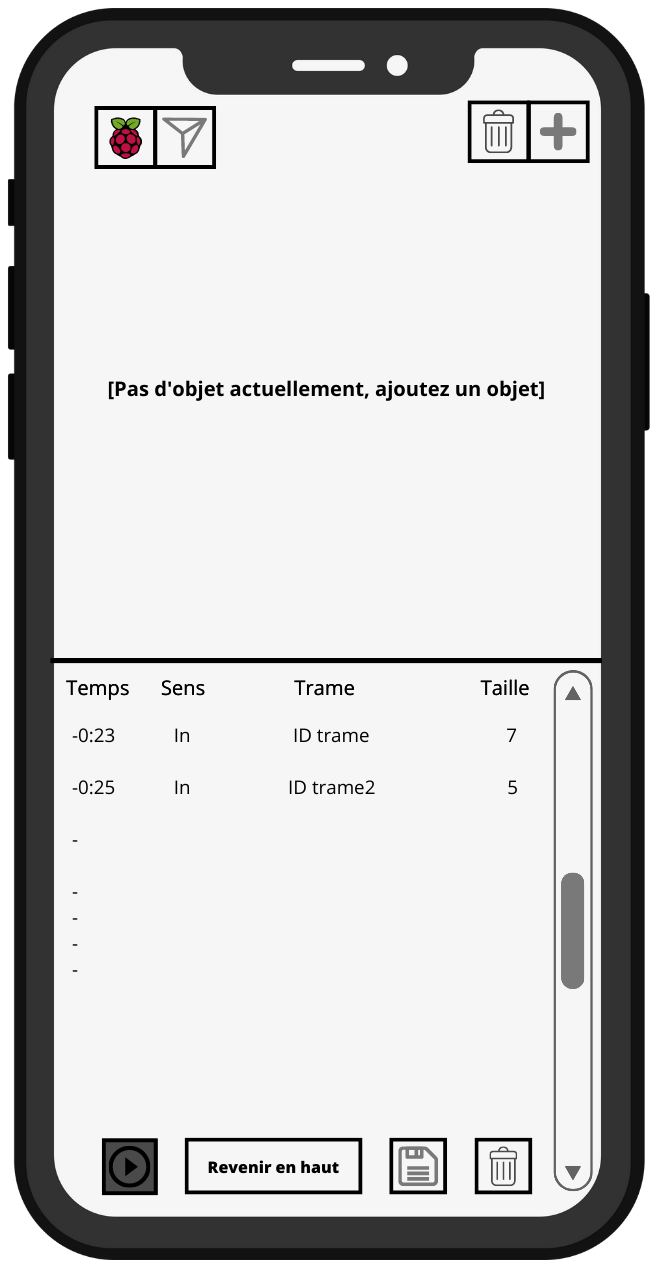
\includegraphics[width=0.5\textwidth]{sections/3_Exigences_specifiques/1_IHM/ihm/ecranPrincipalSansObjet.png}
    \captionof{figure}{Affichage de EcranPrincipal sans objet}
    \label{ecran_sans_objet}
\end{minipage}\hfill 

\newpage

L'ajout d'objet se concrétise en cliquant sur l'icône {\guillemetleft} + {\guillemetright} (bouton [ajouterObjet]) en haut à droite de l'écran. PopupAjoutObjet s'affiche alors pour que Utilisateur insère un nouveau nom d'objet (voir figure \ref{ecran_creation_objet}). Lorsque le nom est entré, Utilisateur clique sur {\guillemetleft} Ajouter {\guillemetright} (bouton [validerAjoutObjet]) pour valider l'ajout de l'objet et l'afficher automatiquement dans la liste des objets présents sur l'application {\nomApplication}. \newline \\ 
Si Utilisateur ne remplit pas le champ du nom d'objet lors de la création d'un nouvel objet dans l'application {\nomApplication}, celle-ci va automatiquement créer un objet avec un nom d'objet par défaut prérempli. Ce nom d'objet par défaut est visible en italique et en gris dans le champ nommé <champNomObjet> (voir section \ref{dictionnaire}). \\

\begin{minipage}{1\linewidth}
    \centering
    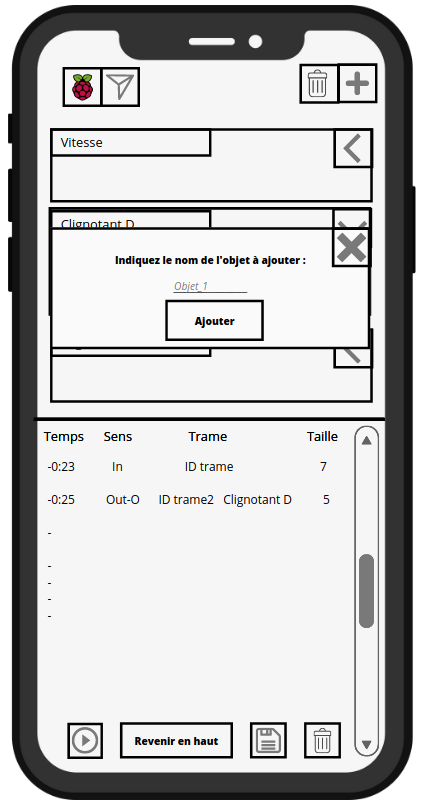
\includegraphics[width=0.5\textwidth]{sections/3_Exigences_specifiques/1_IHM/ihm/ecranCreationObjet.png}
    \captionof{figure}{Affichage de PopupAjoutObjet}
    \label{ecran_creation_objet}
\end{minipage}\hfill 

\newpage

Cependant, Utilisateur ne peut pas utiliser un nom déjà existant lorsqu'il ajoute un objet. Si le nom est déjà pris, un message d'erreur {\guillemetleft} Vous ne pouvez pas ajouter cet objet, le nom existe déjà {\guillemetright} s'affiche (voir figure \ref{ecran_creation_erreur_objet}). \newline \\ De plus, Utilisateur est limité dans le nombre d'objets qu'il peut créer sur l'application CANdroid. Si cette limite est atteinte et que Utilisateur souhaite ajouter un nouvel objet, une fenêtre d'erreur appelée PopupErreurNombreObjet s'affichera (voir figure \ref{ecran_principal_popup_erreur_nombre_objet}). \\\\

\begin{minipage}{0.5\linewidth}
    \centering
    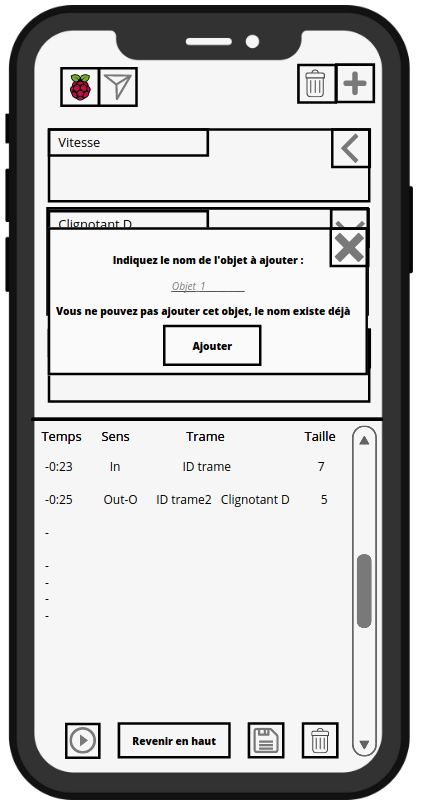
\includegraphics[width=0.7\textwidth]{sections/3_Exigences_specifiques/1_IHM/ihm/ecranCreationObjetErreur.png}
    \captionsetup{justification=centering}
    \captionof{figure}{Affichage de PopupErreurAjoutObjet}
    \label{ecran_creation_erreur_objet}
\end{minipage} \hfill
\begin{minipage}{0.5\linewidth}
    \centering
    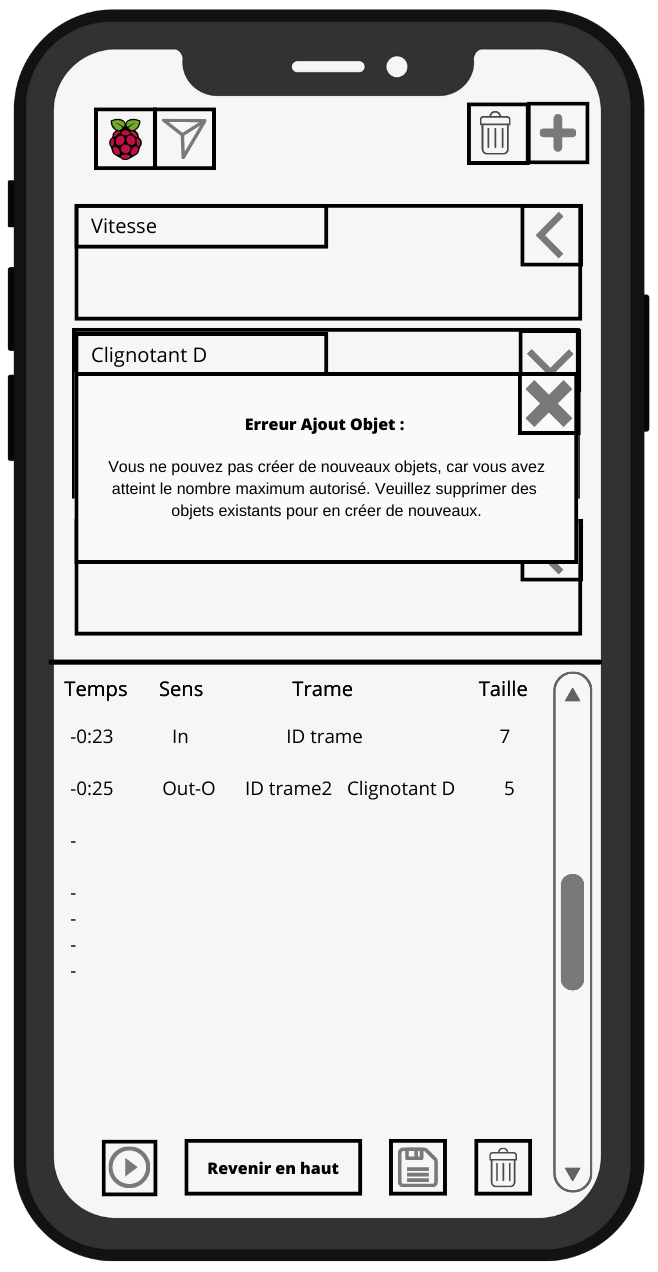
\includegraphics[width=0.7\textwidth]{sections/3_Exigences_specifiques/1_IHM/ihm/ecranErreurNombreObjet.png}
    \captionsetup{justification=centering}
    \captionof{figure}{Affichage de \newline PopupErreurNombreObjet}
    \label{ecran_principal_popup_erreur_nombre_objet}
\end{minipage} 

\newpage

Pour supprimer un objet, Utilisateur clique sur l'objet, la case entière se grise puis Utilisateur clique sur la poubelle en haut à droite de EcranPrincipal (bouton [suppressionElement] sur la figure \ref{ecran_objet_selectionne}). PopupSuppressionElement s'affiche pour demander confirmation à Utilisateur. La suppression d'un objet entraîne la suppression des trames associées à cet objet. La liste des éléments sélectionnés à supprimer est indiquée sur le pop-up et Utilisateur clique sur {\guillemetleft} Supprimer {\guillemetright} (bouton [validerSuppressionElement]) pour valider la suppression (voir figure \ref{ecran_suppression_element}).
 
\vspace{0.5cm}
\begin{minipage}{0.5\linewidth}
    \centering
    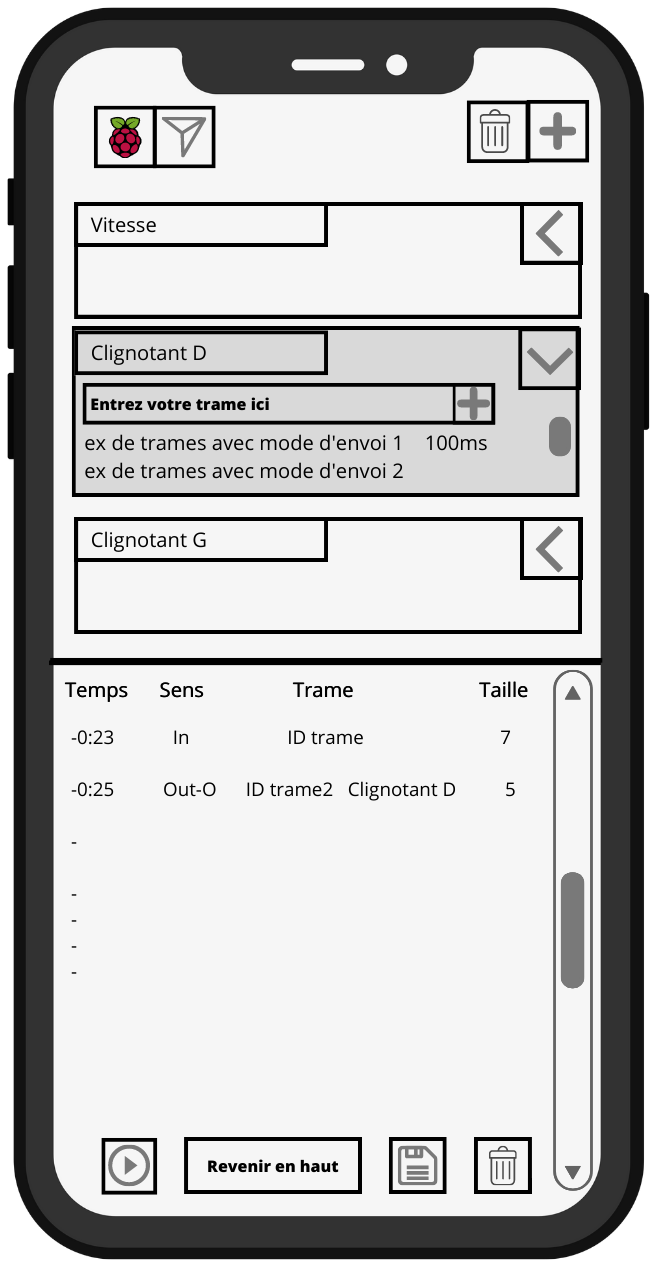
\includegraphics[width=0.7\textwidth]{sections/3_Exigences_specifiques/1_IHM/ihm/ecranPrincipalSelectionObjet.png}
    \captionsetup{justification=centering}
    \captionof{figure}{Affichage de EcranPrincipal\newline avec l'objet {\guillemetleft} Clignotant D {\guillemetright} sélectionné} \label{ecran_objet_selectionne}
\end{minipage}\hfill
\begin{minipage}{0.5\linewidth}
    \centering
    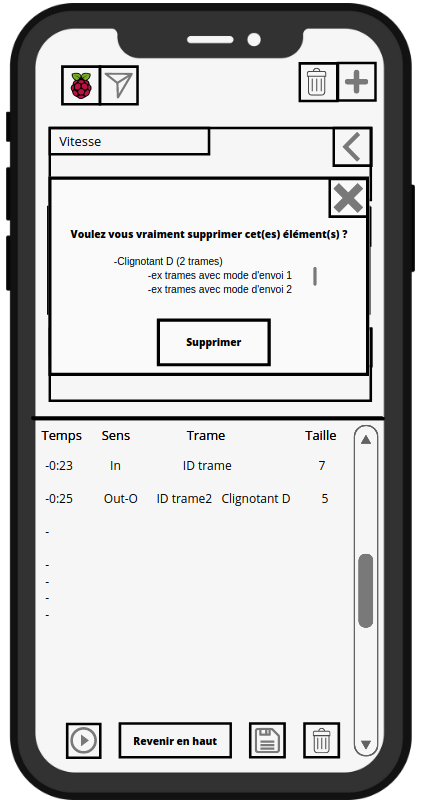
\includegraphics[width=0.7\textwidth]{sections/3_Exigences_specifiques/1_IHM/ihm/ecranSuppressionElementObjet.png}
    \captionsetup{justification=centering}
    \captionof{figure}{Affichage de PopupSuppressionElement} \label{ecran_popup_suppression_element}
\end{minipage} \newline 

\newpage
\textbf{Trames : } \\

Chaque trame est associée à un objet. Les trames sont visibles dans le rectangle de l'objet associé à la suite du nom de l'objet et dans l'ordre de leur ajout. Si possible, la trame est affichée dans sa globalité. Une trame possède un mode d'envoi : cyclique ou ponctuel. 
Pour visualiser la liste des trames, Utilisateur clique sur la flèche de l'objet (bouton [deplierMenuObjet]) pour dérouler le menu de l'objet et ainsi voir ses trames. Voir sur la figure \ref{ecran_principal} où le menu de l'objet {\guillemetleft} Clignotant D {\guillemetright} est déroulé et on peut y voir ses trames, contrairement à l'objet {\guillemetleft} Vitesse {\guillemetright}. \newline

\begin{minipage}{0.5\linewidth}
    \centering
    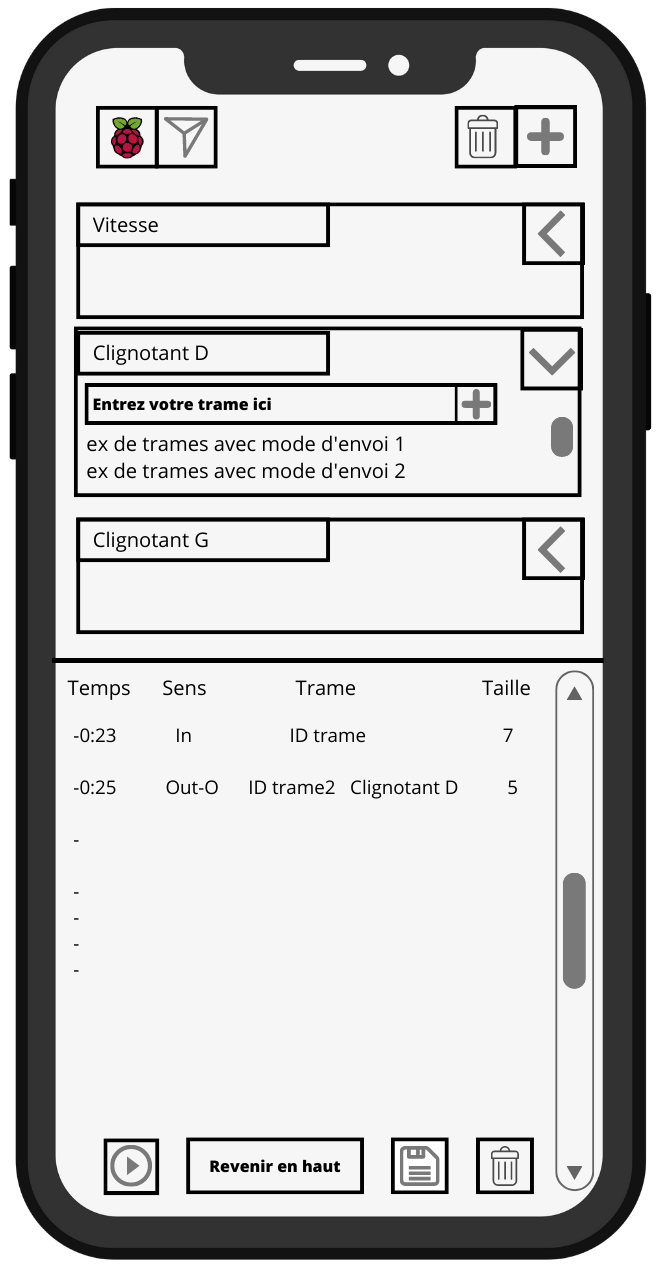
\includegraphics[width=0.7\textwidth]{sections/3_Exigences_specifiques/1_IHM/ihm/ecranPrincipal.png}
    \captionsetup{justification=centering}
    \captionof{figure}{Affichage de EcranPrincipal\newline pour la saisie de trames} 
    \label{ecran_principal_ajout_trame}
\end{minipage}\hfill
\begin{minipage}{0.5\linewidth}
    \centering
    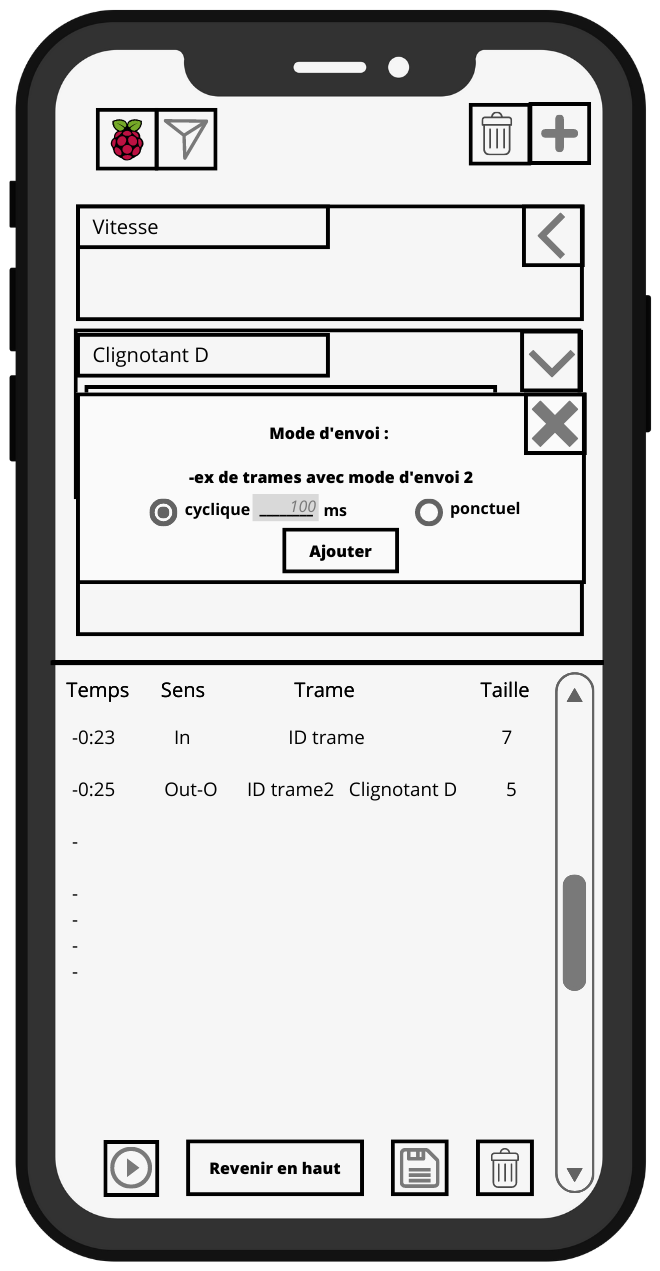
\includegraphics[width=0.7\textwidth]{sections/3_Exigences_specifiques/1_IHM/ihm/ecranModeEnvoiTrame.png}
    \captionsetup{justification=centering}
    \captionof{figure}{Affichage de PopupModeEnvoiTram} 
    \label{ecran_mode_envoi_trames}
\end{minipage} \newline 

\vspace{0.5cm}

Pour ajouter une nouvelle trame, Utilisateur se place dans l'objet auquel il veut l'associer. Il saisit la trame sous le format {\guillemetleft} \#id\$size\@@message {\guillemetright} dans champ <champTrame>. C'est à Utilisateur d'écrire à la main les séparateurs. Cette syntaxe permet d'éviter à Utilisateur d'écrire les zéros non-significatifs. Utilisateur clique ensuite sur le bouton [ajouterTrame]. Si Utilisateur ne saisit pas la trame sous le bon format, PopupErreurSaisieTrame s'affiche (voir figure \ref{ecran_principal_popup_erreur_saisie_trame}). Tant que Utilisateur ne saisit pas une trame sous le bon format, l'ajout ne pourra pas se faire.
\newline \\
Lorsque Utilisateur entre le bon format défini précédemment pour les trames, PopupModeEnvoiTrame s'ouvre (voir figure \ref{ecran_mode_envoi_trames}) et demande à Utilisateur de choisir le mode d'envoi de la trame, pour cela, il doit cliquer sur le bouton radio correspondant au mode d'envoi souhaité. Un radio bouton est un élément qui permet à Utilisateur de sélectionner le mode d'envoi ponctuel (bouton [radioBoutonPonctuel]) ou le mode d'envoi cyclique (bouton [radioBoutonCyclique]). Lorsqu'un bouton radio est sélectionné, le cercle le définissant se remplit, et l'autre bouton radio est automatiquement désélectionné, le cercle le définissant se vide. Par défaut, une trame est périodique de périodicité 100ms mais Utilisateur peut la modifier grâce au champ <champPeriodicite>. Utilisateur clique sur {\guillemetleft} Ajouter {\guillemetright} (bouton [validerModeEnvoi]) pour valider l'ajout de la trame (voir figure \ref{ecran_mode_envoi_trames}). \newline

De la même manière que pour l'ajout d'objets, il existe également une limite pour le nombre de trames que Utilisateur peut ajouter. Si cette limite est atteinte et que Utilisateur tente d'ajouter une nouvelle trame, PopupErreurNombreTrame s'affiche (voir figure \ref{ecran_principal_popup_erreur_nombre_trame}).
\newline \\

\begin{minipage}{0.5\linewidth}
    \centering
    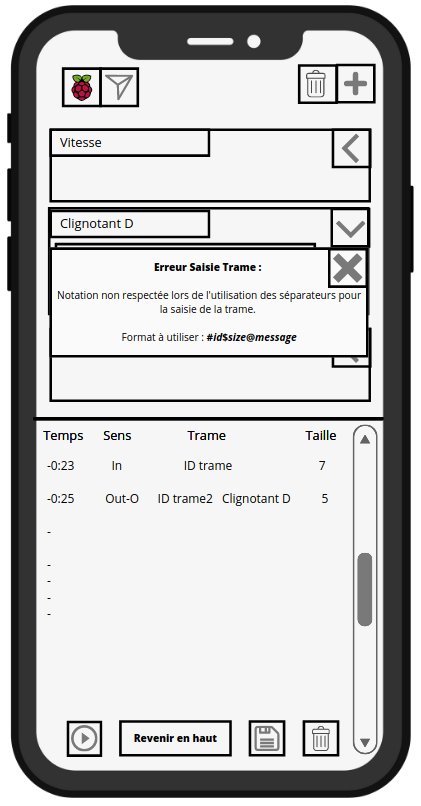
\includegraphics[width=0.7\textwidth]{sections/3_Exigences_specifiques/1_IHM/ihm/ecranErreurTrame.png}
    \captionsetup{justification=centering}
    \captionof{figure}{Affichage de\newline PopupErreurSaisieTrame} 
    \label{ecran_principal_popup_erreur_saisie_trame}
\end{minipage}\hfill
\begin{minipage}{0.5\linewidth}
    \centering
    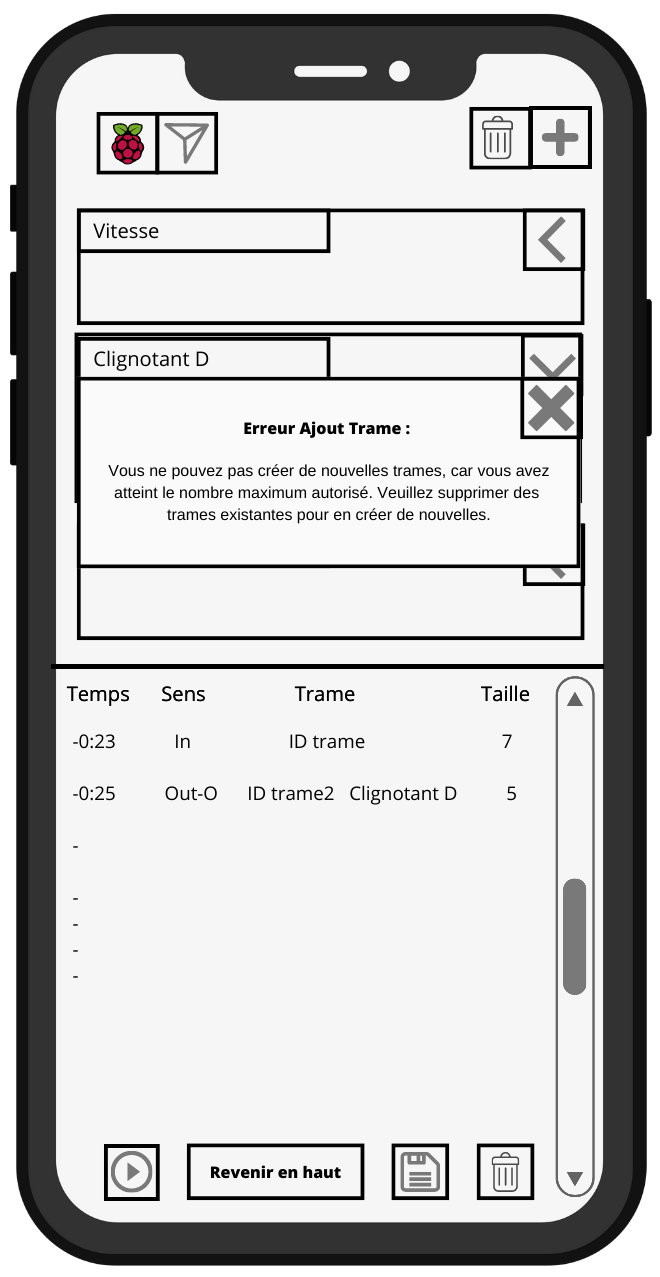
\includegraphics[width=0.7\textwidth]{sections/3_Exigences_specifiques/1_IHM/ihm/ecranErreurNombreTrame.png}
    \captionsetup{justification=centering}
    \captionof{figure}{Affichage de PopupErreurNombreTrame} 
    \label{ecran_principal_popup_erreur_nombre_trame}
\end{minipage} \newline 

\newpage

Pour envoyer une trame, Utilisateur clique sur une trame à envoyer. S'il souhaite en envoyer plusieurs, la sélection est successive. Une trame est considérée comme sélectionnée si elle est grisée claire (voir figure \ref{ecran_trame_selectionne}). Si Utilisateur souhaite désélectionner une trame, il lui suffit de re-cliquer dessus. Lorsque la sélection est effectuée, Utilisateur clique sur l'icône d'envoi en haut à gauche de l'écran (bouton [lancerEnvoi]). Une trame en cours d'envoi se distingue par un surlignage gris foncé et l'écriture en blanc (voir figure \ref{ecran_trame_envoi}). Le bouton d'envoi est également blanc sur fond gris foncé pour indiquer que des trames sont en cours d'envoi. Dans cet état-là, les boutons de suppression et d'ajout (trames comme objets) sont en noir sur fond gris foncé pour montrer que les outils correspondants sont désactivés.
\\\\
\vspace{2cm}
\begin{minipage}{0.5\linewidth}
    \centering
    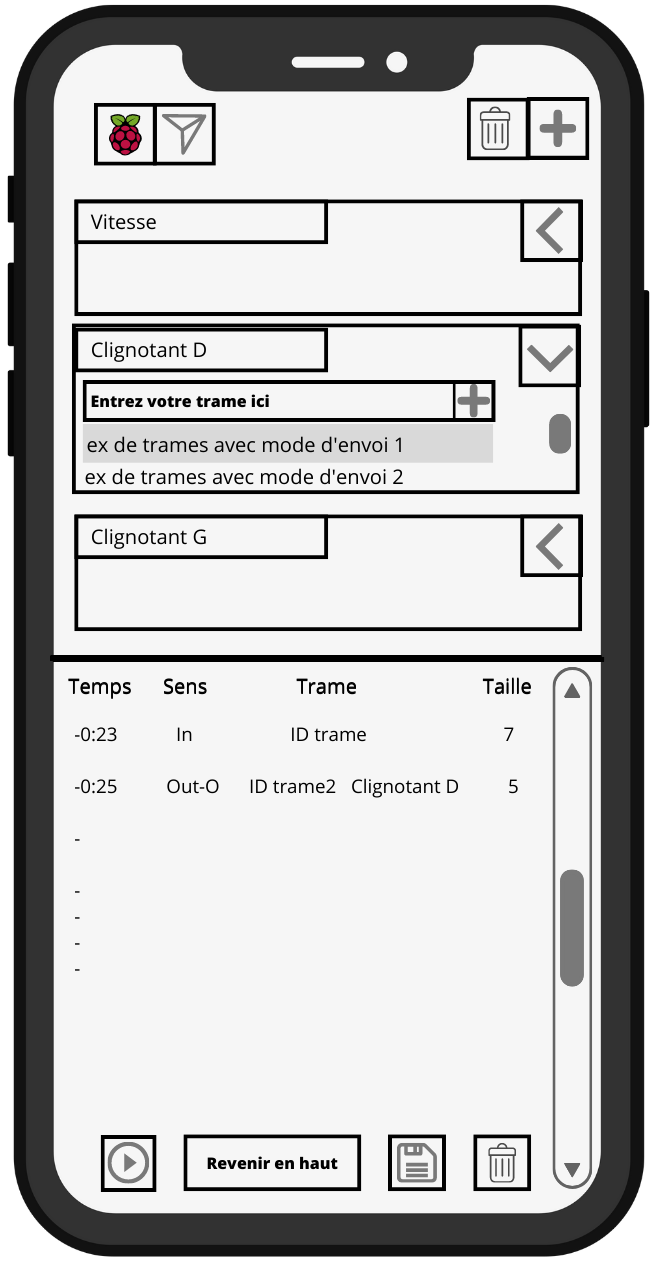
\includegraphics[width=0.7\textwidth]{sections/3_Exigences_specifiques/1_IHM/ihm/ecranPrincipalSelectionTrame.png}
    \captionsetup{justification=centering}
    \captionof{figure}{Affichage de EcranPrincipal\newline avec  une trame de l'objet {\guillemetleft} Clignotant D {\guillemetright} sélectionnée}
    \label{ecran_trame_selectionne}
\end{minipage}\hfill
\begin{minipage}{0.5\linewidth}
    \centering
    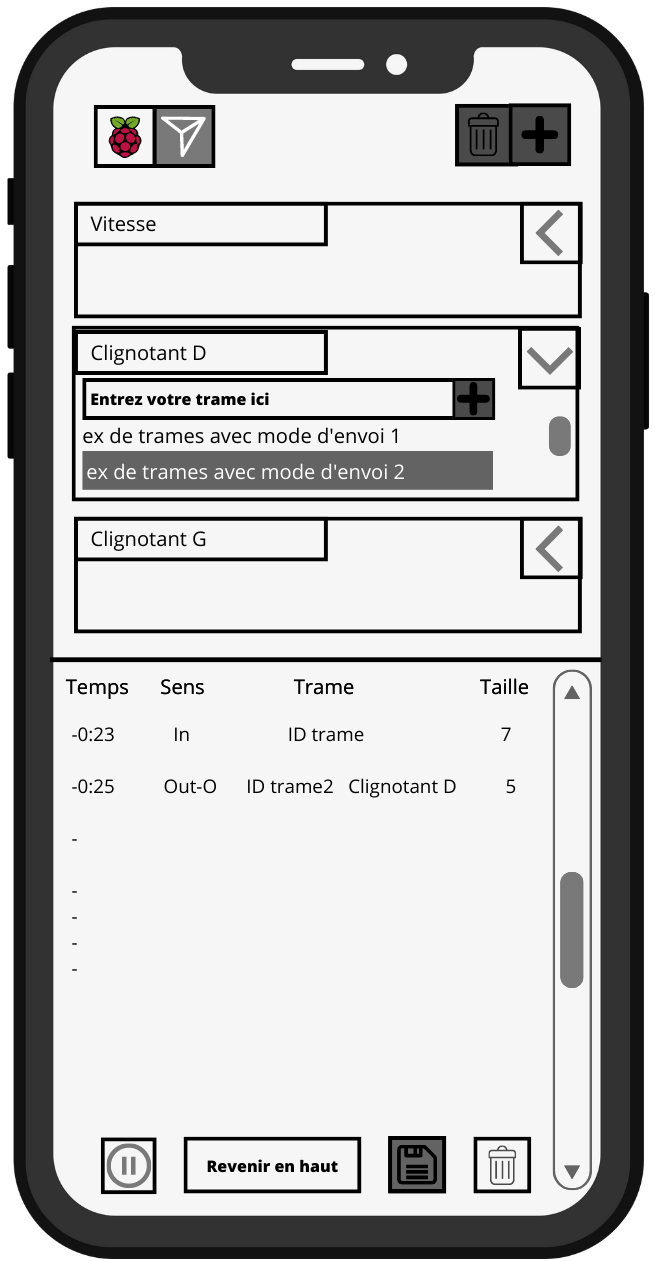
\includegraphics[width=0.7\textwidth]{sections/3_Exigences_specifiques/1_IHM/ihm/ecranPrincipalTrameEnCours.png}
    \captionsetup{justification=centering}
    \captionof{figure}{Affichage de EcranPrincipal lorsque des trames sont en cours d'envoi}
    \label{ecran_trame_envoi}
\end{minipage} \newline 
\vspace{1cm}

\newpage
Pour arrêter l'envoi des trames, Utilisateur clique à nouveau sur le bouton d'envoi (bouton [arreterEnvoi]), PopupArretEnvoi apparaît pour demander la confirmation à Utilisateur (voir figure \ref{ecran_arret_envoi}). Utilisateur valide ce changement d'état en cliquant sur {\guillemetleft} Oui {\guillemetright} (bouton [validerArretEnvoi]), dans le cas inverse Utilisateur clique sur {\guillemetleft} Non {\guillemetright} (bouton [annulerArretEnvoi]) et le mode d'envoi continue. 
\\\\
\begin{minipage}{1\linewidth}
    \centering
    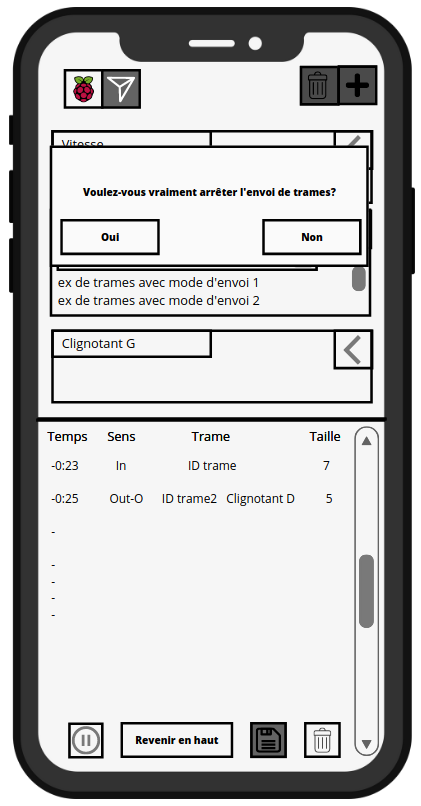
\includegraphics[width=0.48\textwidth]{sections/3_Exigences_specifiques/1_IHM/ihm/ecranArretEnvoi.png}
    \captionof{figure}{Affichage de PopupArretEnvoi}
    \label{ecran_arret_envoi}
\end{minipage}\hfill

\newpage
De même que pour supprimer un objet, pour supprimer une trame, Utilisateur clique sur la trame qu'il souhaite supprimer, la ligne se grise puis Utilisateur clique sur la poubelle (bouton [suppressionElement]) en haut à droite de EcranPrincipal (voir figure \ref{ecran_trame_selectionne}). La liste des éléments sélectionnés à supprimer est indiquée sur PopupSuppressionElement et Utilisateur clique sur {\guillemetleft} Supprimer {\guillemetright} (bouton [validerSuppressionElement]) pour valider la suppression (voir figure \ref{ecran_suppression_trames}).
\\\\
\begin{minipage}{1\linewidth}
    \centering
    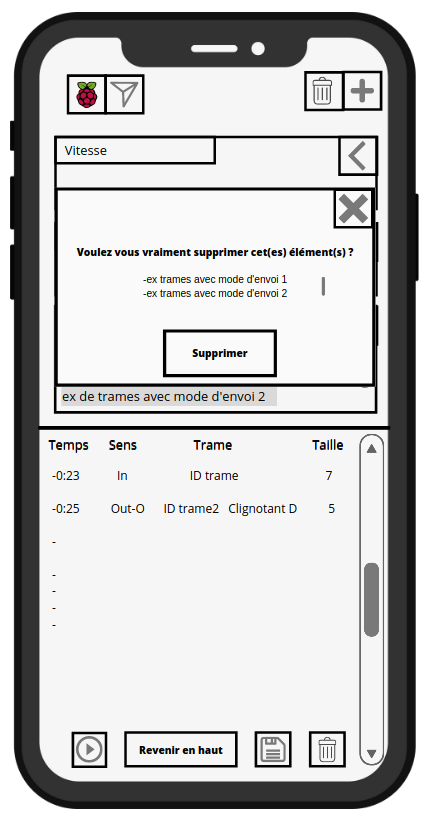
\includegraphics[width=0.45\textwidth]{sections/3_Exigences_specifiques/1_IHM/ihm/ecranSuppressionElementTrame.png}
    \captionsetup{justification=centering}
    \captionof{figure}{Affichage de PopupSuppressionElement \\ avec suppression de trames seulement}
    \label{ecran_suppression_trames}
\end{minipage} \newline
\vspace{1cm}

\newpage
\paragraph{Partie basse de l'écran}
La partie sniffer (partie basse de l'écran) présente les trames CAN envoyées et reçues par la Raspberry Pi lorsqu'il y en a. Lorsque la Raspberry Pi n'est pas encore connectée, un commentaire indique qu'il n'y a pas de trames actuellement {\guillemetleft} Pas de trame actuellement {\guillemetright} (voir figure \ref{ecran_sans_objet}). 
\newline
Les trames arrivent par le haut du terminal donc la trame la plus récente sera celle du haut. 
Pour chaque trame CAN, on précise la trame (id + donnée), l'objet auquel elle est associée (si la trame est envoyée), sa taille, son sens ({\guillemetleft} In {\guillemetright} correspond à la réception sur l'application {\nomApplication} et {\guillemetleft} Out {\guillemetright} correspond à l'émission depuis l'application {\nomApplication}) et un repère temporel. L'envoi d'une trame cyclique se remarque par l'ajout du symbole O dans son sens (Out-O).
La trame est au format {\guillemetleft} \#id\$size\@@message {\guillemetright} avec les caractères {\guillemetleft} \# {\guillemetright}, {\guillemetleft} \$ {\guillemetright} et {\guillemetleft} \@@ {\guillemetright} comme séparateurs.
\newline 
Le repère temporel est en millisecondes, et est initialisé à zéro lorsque la première trame est sniffée sur le bus CAN.
\\\\
\begin{minipage}{0.9\linewidth}
    \centering
    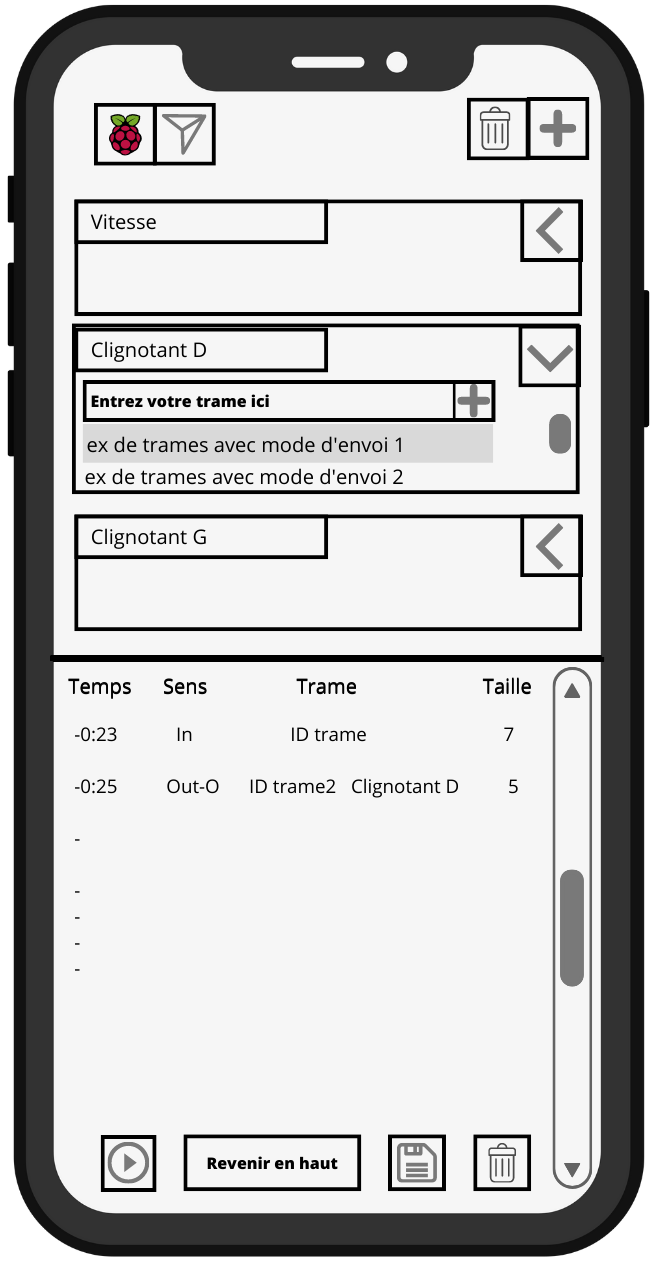
\includegraphics[width=0.45\textwidth]{sections/3_Exigences_specifiques/1_IHM/ihm/ecranPrincipalSelectionTrame.png}
    \captionof{figure}{Affichage de EcranPrincipal avec le sniffer en mode {\guillemetleft} pause {\guillemetright}}
    \label{ecran_sniffer_pause}
\end{minipage}\hfill

\newpage
Utilisateur peut mettre en pause le sniffer en cliquant sur le bouton pause (bouton [pause]) en bas à gauche de l'écran (voir figure \ref{ecran_sniffer_pause}). Lorsque le sniffer est en pause, Utilisateur peut exporter les trames présentes dans le terminal vers un fichier de log, en cliquant sur l'icône {\guillemetleft} enregistrer {\guillemetright} (bouton [exporterSniffer]) en bas à droite de l'écran. 
Il peut à la suite remettre le sniffer en écoute en cliquant sur l'icône play (bouton [play] sur la figure \ref{ecran_sniffer_pause}). Lorsque le sniffer est en cours de lecture, le bouton pour enregistrer le sniffer est verrouillé d'où le fait qu'il soit en noir sur fond gris foncé (voir figure \ref{ecran_sniffer_play}). 
\\\\
\begin{minipage}{1\linewidth}
    \centering
    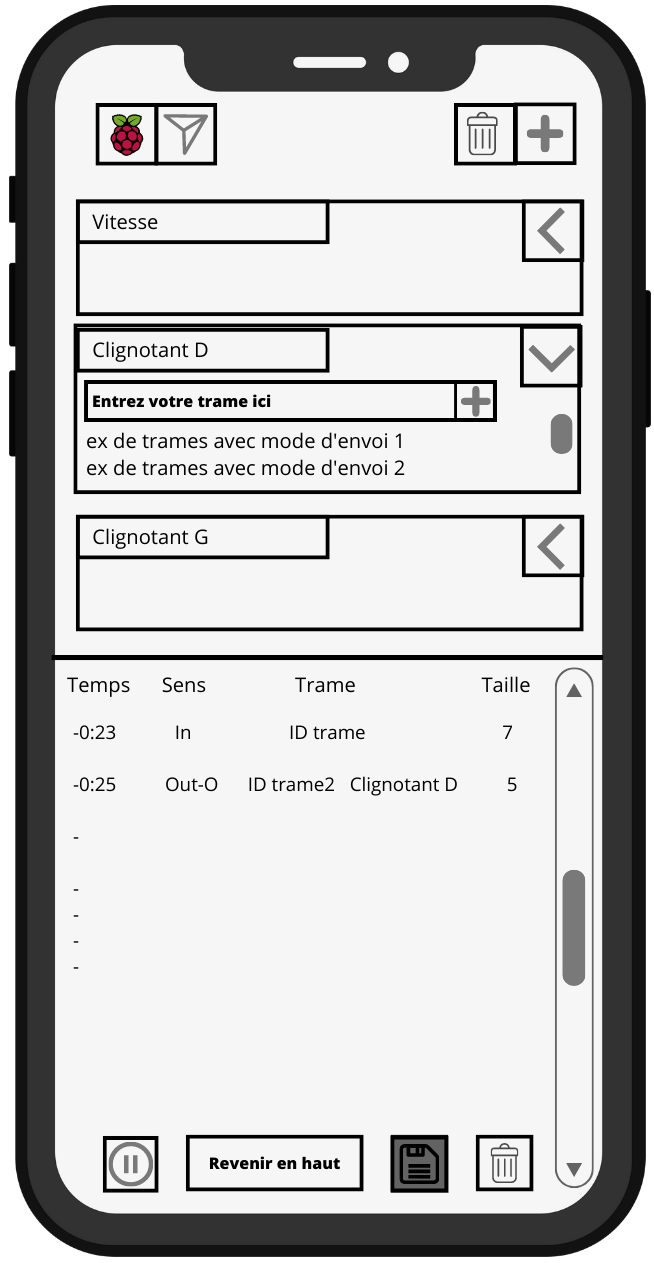
\includegraphics[width=0.4\textwidth]{sections/3_Exigences_specifiques/1_IHM/ihm/ecranSnifferPlay.png}
    \captionsetup{justification=centering}
    \captionof{figure}{Affichage de EcranPrincipal avec le \\ sniffer en mode {\guillemetleft} play {\guillemetright}}
    \label{ecran_sniffer_play}
\end{minipage}\hfill

\vspace{0.5cm}

L'enregistrement contient toutes les informations des trames visibles sur le sniffer. Les trames sont exportées dans un fichier de log (voir section \ref{dictionnaire}).\newline \\
Utilisateur peut revenir en haut de la liste des trames en cliquant sur le bouton [revenirEnHaut], et peut vider le sniffer des trames actuelles en cliquant sur la poubelle en bas de l'écran à droite sur le bouton [viderSniffer] (voir la figure \ref{ecran_sniffer_play}). 
\newpage